\chapter{实验与结果分析}\label{chap:experiments}

\section{引言}\label{sec:ch4-intro}

本章在EGFR、VEGF/VEGFR和IDH1/IDH2三个代表性GBM靶点上对本文提出的GBM候选分子生成框架进行系统性的实验验证。首先介绍实验环境、数据来源、靶点结构准备和分子预处理流程；然后展示主实验结果，分析生成分子在DrugCLIP Score、Vina对接分数、BBB穿透性预测等指标上的表现；接着展示对比实验结果和消融实验结果，分析各模块的贡献；最后对结果进行深入讨论，包括失败样例分析和误差来源讨论。

需要指出的是，本文所使用的DrugCLIP Score、Vina对接分数和BBB穿透性预测分数均属于计算预测指标，主要用于早期虚拟筛选和候选分子排序参考，尚不能替代体外活性测定、hERG阻断实验或PAMPA-BBB渗透实验等实验验证。因此，本文实验结果仅表明相关分子具有进一步验证价值，而不能直接等同于已确认的药效或临床转化潜力。

\section{实验设置}\label{sec:exp-setup}

\subsection{实验环境}\label{sec:exp-env}

本文实验在单机环境下完成，硬件与软件环境配置如表\ref{tab:dependencies}所示。

\begin{table}[htbp]
    \centering
    \caption{实验环境配置}\label{tab:dependencies}
    \begin{tabular}{lll}
        \toprule
        \textbf{类别} & \textbf{配置} & \textbf{说明} \\
        \midrule
        GPU & NVIDIA RTX 3090, 24GB & 模型推理与LoRA微调 \\
        CPU & AMD EPYC 7742 & 数据预处理 \\
        Python & 3.11 & 运行时环境 \\
        PyTorch & 2.x (BF16) & 深度学习推理 \\
        RDKit & Latest & 分子解析与描述符计算 \\
        Transformers & Latest & Qwen2-7B-Instruct加载 \\
        PEFT & Latest & LoRA适配器管理 \\
        AutoDock Vina & 1.2.x & 分子对接 \\
        \bottomrule
    \end{tabular}
\end{table}

\subsection{模型配置}\label{sec:model-config}

\textbf{基础模型}：Qwen2-7B-Instruct~\cite{Qwen2Team2024}，约70亿参数，支持BF16推理。

\textbf{LoRA微调适配器}：\texttt{saves/GBM-PharmaMind-Qwen2-7B-Instruct-Adapter-gbm-with-graph-models}。该适配器在预训练的底层多模态生成模型（Llamole/Qwen2-7B-Instruct）基础上~\cite{liu2025multimodal}，使用本文构建的GBM领域数据集进行LoRA微调~\cite{hu2022lora}。

\textbf{生成超参数配置}：如表\ref{tab:gen-params}所示。

\begin{table}[htbp]
    \centering
    \caption{生成超参数配置}\label{tab:gen-params}
    \begin{tabular}{lll}
        \toprule
        \textbf{参数} & \textbf{值} & \textbf{说明} \\
        \midrule
        max\_length & 1024 & 输入+输出的最大token数 \\
        max\_new\_tokens & 256 & 最大生成token数 \\
        temperature & 0.7 & 采样温度，控制随机性 \\
        top\_p & 0.9 & Nucleus采样参数 \\
        do\_sample & True & 启用采样 \\
        num\_return\_sequences & 5 & 每次生成候选数 \\
        \bottomrule
    \end{tabular}
\end{table}

为保证实验可复现性，本文在模型推理和分子生成过程中设置了随机种子控制。温度采样时仍存在少量随机性，这在分子生成任务中是预期且有益的~\cite{Bagal2021}，有助于增加生成分子的多样性~\cite{Zhou2019Exp}。

\section{靶点结构准备与对接设置}\label{sec:target-prep}

分子对接的准确性高度依赖于靶点蛋白结构的准备质量。本节描述靶点结构的来源和预处理流程。

\subsection{靶点蛋白结构来源}\label{sec:protein-source}

本文实验中使用的EGFR、VEGFR2和IDH1蛋白结构来源于RCSB蛋白质数据库（PDB）的晶体结构文件。靶点结构的选取遵循以下原则：（1）选取高分辨率（$\le$ 3.0 \AA）的晶体结构，确保蛋白结构清晰~\cite{Trott2010}；（2）选取含有与靶点结合的小分子配体的结构，便于确定对接盒子中心~\cite{Trott2010}；（3）优先选取与GBM相关的突变体结构（如IDH1 R132H突变体）。

\subsection{靶点结构预处理}\label{sec:protein-prep}

靶点结构的预处理流程包括以下步骤：

\begin{enumerate}
    \item \textbf{加水与加氢}：使用MGLTools对蛋白结构进行极性氢原子添加；
    \item \textbf{去除水分子}：删除结晶水分子，避免干扰对接；
    \item \textbf{配体处理}：保留原配体作为口袋定位参考；
    \item \textbf{原子电荷处理}：为蛋白和配体原子分配力场电荷；
    \item \textbf{格式转换}：转换为PDBQT格式供AutoDock Vina使用。
\end{enumerate}

对于Vina对接失败的分子（分子无法放入盒子或能量最小化不收敛），本文在统计中标记为"对接失败"。对接失败可能由以下原因导致：（1）生成分子的柔性强或体积过大，无法在给定对接盒子内完成构象搜索~\cite{Trott2010}；（2）生成分子含有金属离子或特殊基团，与力场参数不兼容~\cite{Trott2010}。对接失败的分子不进入后续的Vina分数统计，但在DrugCLIP统计中仍保留。

\subsection{对接盒子参数}\label{sec:docking-box}

对接盒子参数决定了配体-受体对接的空间范围~\cite{Trott2010}。盒子中心基于原配体位置确定~\cite{Trott2010}。

\begin{itemize}
    \item \textbf{盒子尺寸}：22.5 $\times$ 22.5 $\times$ 22.5 \AA$^3$~\cite{Trott2010}。22.5 \AA\ 的盒子尺寸能够容纳大多数中等大小的GBM相关分子配体~\cite{Trott2010}。
    \item \textbf{Vina exhaustiveness}：设置为8（默认），控制对接搜索的穷尽程度~\cite{Trott2010}。
    \item \textbf{num\_modes}：设置为10，控制每个分子最多输出10个对接构象~\cite{Trott2010}。
    \item \textbf{能量范围}：默认设置~\cite{Trott2010}。
\end{itemize}

\section{分子预处理与有效性过滤}\label{sec:molecule-prep}

生成分子的预处理流程对于保证后续评估的准确性至关重要~\cite{Trott2010}。

\subsection{SMILES解析与标准化}\label{sec:smiles-parse}

分子生成的原始输出为SMILES字符串，需要经过以下处理步骤：

\begin{enumerate}
    \item \textbf{SMILES解析}：使用RDKit解析SMILES字符串；
    \item \textbf{有效性检查}：对解析失败的SMILES（无效化学结构）进行统计和剔除；
    \item \textbf{标准化}：使用RDKit的标准化流程统一同分异构体的表示；
    \item \textbf{去重}：对标准化后的分子集合进行SMILES去重。
\end{enumerate}

SMILES解析失败是分子生成任务中的常见问题~\cite{Bagal2021}。LLM生成的SMILES可能包含语法错误（如未闭合的括号、非法原子符号等），RDKit无法解析这些字符串~\cite{RDKit}。

\subsection{理化性质过滤}\label{sec:physchem-filter}

本文在分子预处理阶段进行基础理化性质过滤，该步骤的目的是剔除明显异常或难以进入后续计算流程的分子结构，保证后续对接和评分流程的可计算性。\section{评估指标体系}\label{sec:eval-metrics}

本文使用的评估指标体系已在第3章详细介绍，本节补充各指标的实验解读和用途区分。

\subsection{DrugCLIP Score}\label{sec:drugclip-metric}

DrugCLIP是一种基于对比学习的分子-靶点结合活性预测模型~\cite{Gao2023}。该模型将蛋白口袋和分子分别映射到统一的向量空间~\cite{Gao2023}，通过计算向量相似度评估蛋白-分子匹配程度~\cite{Gao2023}。正值表示预测有活性，负值表示预测无活性。DrugCLIP Score是语义空间的相似度度量~\cite{Gao2023}，不是实验结合亲和力（Kd/Ki）~\cite{Gao2023}，仅反映在当前模型和数据分布下的相对预测活性~\cite{Gao2023}。若生成分子偏离训练数据分布（如结构高度新颖），预测分数的可靠性可能下降~\cite{Gao2023}。

\subsection{Vina对接分数}\label{sec:vina-metric}

AutoDock Vina对接分数（kcal/mol）是评估配体-受体结合模式的经验打分~\cite{Trott2010}。\textbf{需要说明的是}：Vina分数是经验打分~\cite{Trott2010}，不代表实验结合自由能（$\Delta$G）~\cite{Trott2010}，不能直接用于计算Ki/Kd~\cite{Trott2010}。Vina分数在本文中的定位是"生成阶段剪枝反馈"~\cite{Trott2010}，而非"最终排序依据"~\cite{Gao2023}。

Vina分数的判读标准为：
\begin{itemize}
    \item Vina < -7.0 kcal/mol：对接分数处于较优区间（预设强结合参考阈值~\cite{Trott2010}）
    \item -7.0 $\le$ Vina < -5.0 kcal/mol：中等结合
    \item Vina $\ge$ -5.0 kcal/mol：弱结合，触发硬截断剪枝
\end{itemize}

Vina分数用于：（1）评估生成分子与靶点蛋白的空间匹配程度；（2）通过硬截断阈值过滤明显不匹配的分子；（3）作为MPO Reward的一个组成部分参与生成阶段反馈。

\subsection{ADMET性质}\label{sec:bbb-metric}

TotalScore 中的 ADMET 性质指标（bbb\_norm、pains\_brenk\_alert、pgp\_risk、SA\_score、physchem\_score）均通过 SwissADME 网站测得。SwissADME 是常用的免费在线药物性质预测工具，可快速返回类药性评估、BBB 穿透倾向、PAINS/Brenk 结构警报、P-gp 外排泵风险及合成可及性等多项指标。\textbf{需要说明的是}：SwissADME 预测结果均为计算估算值~\cite{Daina2017}，\textit{不代表实际实验测定值}，预测偏差需结合实验进一步验证~\cite{Daina2017}。

\subsection{综合Score与分层层级}\label{sec:total-score}

TotalScore用于生成完成后的离线综合排序，对所有通过生成流程得到的分子进行重新打分，不参与生成阶段剪枝。该指标采用加权算术平均，并将结果映射到0—100分区间。TotalScore的指标来源包括DrugCLIP预测活性、外部工具重新计算的Vina对接分数、BBB穿透性预测、SA合成可及性、PAINS/Brenk结构警报、P-gp风险以及基础理化性质等，用于对候选分子进行最终优先级排序。

\begin{equation}
\begin{aligned}
    \text{DrugCLIP\_norm} &= \frac{\max(\text{DrugCLIP}, 0)}{3.0} \\
    \text{综合Score} &= 0.30 \times \text{DrugCLIP\_norm} + 0.30 \times \text{vina\_norm} \\
                     &\quad + 0.15 \times \text{bbb\_norm} + 0.07 \times (1-\text{pains\_brenk\_alert}) \\
                     &\quad + 0.05 \times (1-\text{pgp\_risk}) + 0.05 \times \text{SA\_score} \\
                     &\quad + 0.08 \times \text{physchem\_score}
\end{aligned}
\end{equation}

分层层级定义如表\ref{tab:scoring-layers}所示。

\begin{table}[htbp]
    \centering
    \caption{分层层级定义}\label{tab:scoring-layers}
    \begin{tabular}{lll}
        \toprule
        \textbf{层级} & \textbf{Score范围} & \textbf{含义} \\
        \midrule
        高优先级 & Score $\ge$ 80 & 综合指标优秀，建议优先虚拟筛选 \\
        建议验证 & 70 $\le$ Score < 80 & 综合指标良好，值得进一步研究 \\
        保留观察 & 60 $\le$ Score < 70 & 基本达标，需进一步优化 \\
        优先淘汰 & Score < 60 & 多项指标未达标 \\
        \bottomrule
    \end{tabular}
\end{table}

\section{实验靶点与数据}\label{sec:targets}

本文选择三个代表性GBM靶点进行验证，各靶点的选择依据如下：

\begin{itemize}
    \item \textbf{EGFR}：GBM中最常见的突变基因（约40\%），具有重要临床意义~\cite{Fu2025}。EGFR靶点的分子设计需同时考虑 GBM 中常见的 EGFR 扩增、EGFRvIII 变体及其相关旁路信号激活~\cite{Fu2025}。EGFR是GBM中研究较成熟的靶点，已有较多EGFR抑制剂结构和母核信息~\cite{Fu2025}，因此通用模型可能已经学到较多EGFR相关结构模式。
    \item \textbf{VEGF/VEGFR}：驱动GBM肿瘤血管生成~\cite{Fu2025}，是抗血管生成疗法的核心靶点~\cite{Fu2025}。VEGF/VEGFR靶点结合口袋和机制复杂~\cite{Fu2025}，Vina分数波动可能较大。
    \item \textbf{IDH1/IDH2}：GBM的重要分子标志物（约10\%）~\cite{Fu2025}，IDH突变与预后密切相关~\cite{Fu2025}。IDH1突变体口袋结构相对明确~\cite{Fu2025}，可能更适合对接和模型学习~\cite{Fu2025}。
\end{itemize}

\textbf{实验目的}：通过在三个不同特点的靶点上进行实验，验证本文方法在不同靶点类型上的适用性，并分析各靶点的预测结果差异。

\section{主实验结果}\label{sec:main-results}

\subsection{综合Score分布}\label{sec:score-dist}

图\ref{fig:score-dist}展示了生成分子的综合评分分布直方图。

\begin{figure}[htbp]
    \centering
    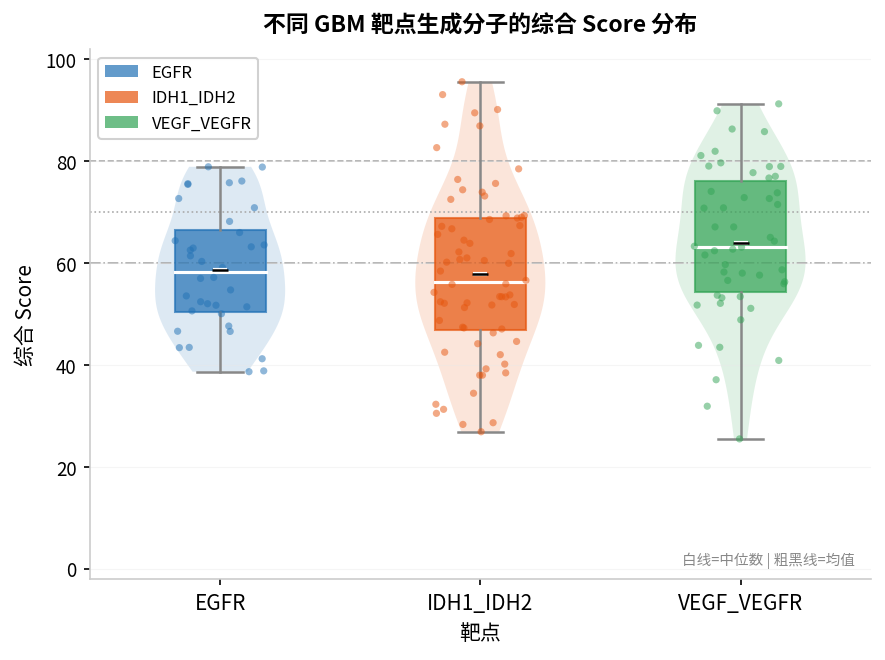
\includegraphics[width=0.8\textwidth]{图片/实验结果可视化图/fig1_score_distribution.zh.png}
    \caption{综合Score分布直方图}\label{fig:score-dist}
\end{figure}

\textbf{结果分析}：VEGF/VEGFR的综合Score分布较为均衡，均值和中位数均高于其他两组，提示该靶点在本计算评价体系下候选分子质量分布更为集中；EGFR和IDH1的分布宽度较窄，整体评分偏低，提示这两个靶点在本框架下的生成分子多集中于中低分层级。

这一分布差异的可能原因包括：（1）VEGF/VEGFR靶点的生成分子在理化性质上更接近CNS药物的典型特征~\cite{Ertl2000,Pardridge2012}；（2）EGFR靶点的成熟度高~\cite{Fu2025}，但同时也需要更复杂的约束设计~\cite{Fu2025}，在当前框架下生成高质量EGFR配体的难度较大；（3）IDH1靶点的结构约束特殊~\cite{Fu2025}，可能需要更精细的骨架设计。

\subsection{DrugCLIP Score分布}\label{sec:drugclip-dist}

图\ref{fig:drugclip-dist}展示了三个靶点生成分子的DrugCLIP Score分布直方图。

\begin{figure}[htbp]
    \centering
    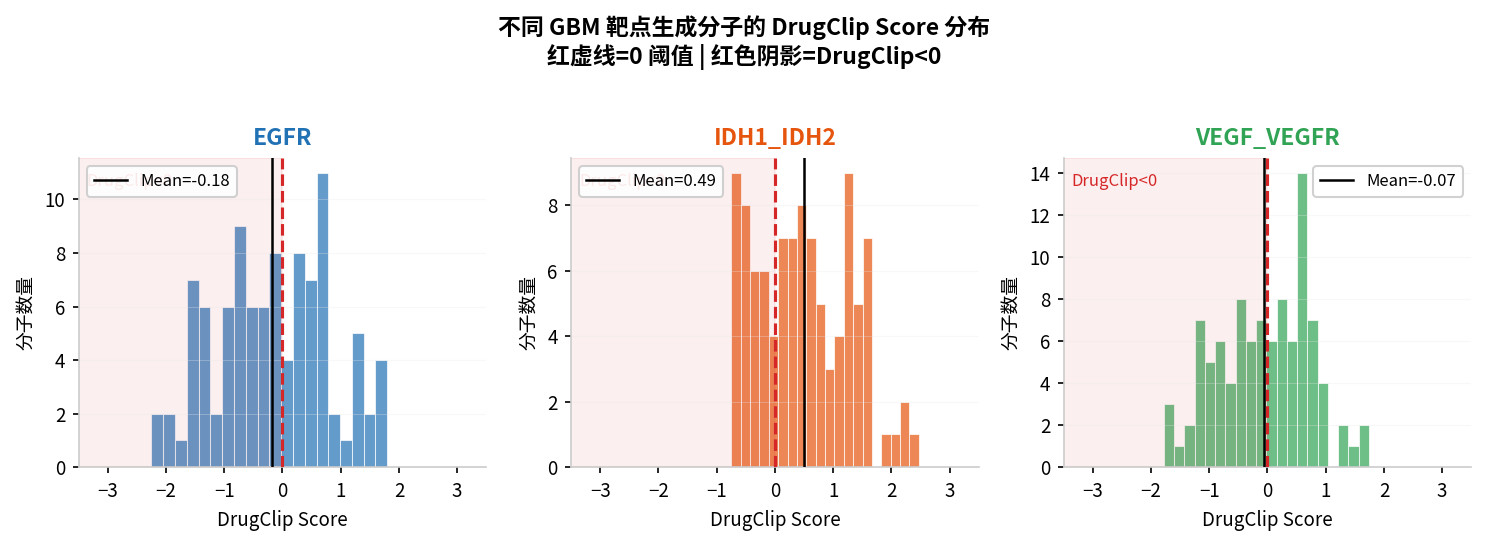
\includegraphics[width=0.8\textwidth]{图片/实验结果可视化图/fig2_drugclip_distribution.zh.png}
    \caption{DrugCLIP Score分布直方图}\label{fig:drugclip-dist}
\end{figure}

\begin{table}[htbp]
    \centering
    \caption{DrugCLIP Score统计数据}\label{tab:drugclip-stats}
    \begin{tabular}{lcccc}
        \toprule
        \textbf{靶点} & \textbf{DrugCLIP>0分子数} & \textbf{均值} & \textbf{标准差} & \textbf{最高值} \\
        \midrule
        EGFR & 43 & 0.57 & 0.37 & 1.61 \\
        IDH1 & 67 & \textbf{0.93} & 0.60 & \textbf{2.47} \\
        VEGF & 48 & 0.62 & 0.38 & 1.74 \\
        \textbf{三靶点合计} & \textbf{158} & \textbf{0.74} & - & - \\
        \bottomrule
    \end{tabular}
\end{table}

\textbf{结果分析}：IDH1靶点的DrugCLIP均值最高（0.93），是三个靶点中预测活性最为突出的~\cite{Gao2023}。这一现象可能与以下因素有关：（1）IDH1靶点的训练数据相对丰富~\cite{Gao2023}；（2）IDH1突变位点（R132H）的口袋结构相对规则~\cite{Fu2025}，适合DrugCLIP模型的语义匹配~\cite{Gao2023}；（3）IDH1生成分子的理化性质更接近训练数据分布~\cite{Gao2023}。

从医学背景来看~\cite{Fu2025}，IDH1/IDH2是GBM分子分型的重要标志物，约10\%的GBM携带IDH突变~\cite{Fu2025}。IDH1突变体通过产生2-羟基戊二酸（2-HG）影响肿瘤代谢~\cite{Fu2025}。由于IDH1在GBM中的重要性已有较多研究~\cite{Fu2025}，相关抑制剂结构信息较为丰富~\cite{Fu2025}，这可能使得模型能够学习到较为有效的分子模式。

\textbf{靶点差异分析}：EGFR的DrugCLIP均值（0.57）相对较低，可能原因包括：（1）EGFR是GBM中研究最成熟的靶点~\cite{Fu2025}，已有大量结构和抑制剂数据~\cite{Fu2025}，模型可能倾向于生成与已知化合物相似的结构，导致与训练数据的差异较大~\cite{Gao2023}；（2）EGFR靶向治疗在GBM中面临 BBB 穿透受限、EGFRvIII 等异常形式以及旁路信号激活等多重挑战~\cite{Fu2025}，在满足这些复杂约束的同时保持高预测活性具有较大难度~\cite{Fu2025}。

\subsection{Vina对接分数分布}\label{sec:vina-dist}

图\ref{fig:vina-dist}展示了DrugCLIP>0分子的Vina对接分数分布箱线图。

\begin{figure}[htbp]
    \centering
    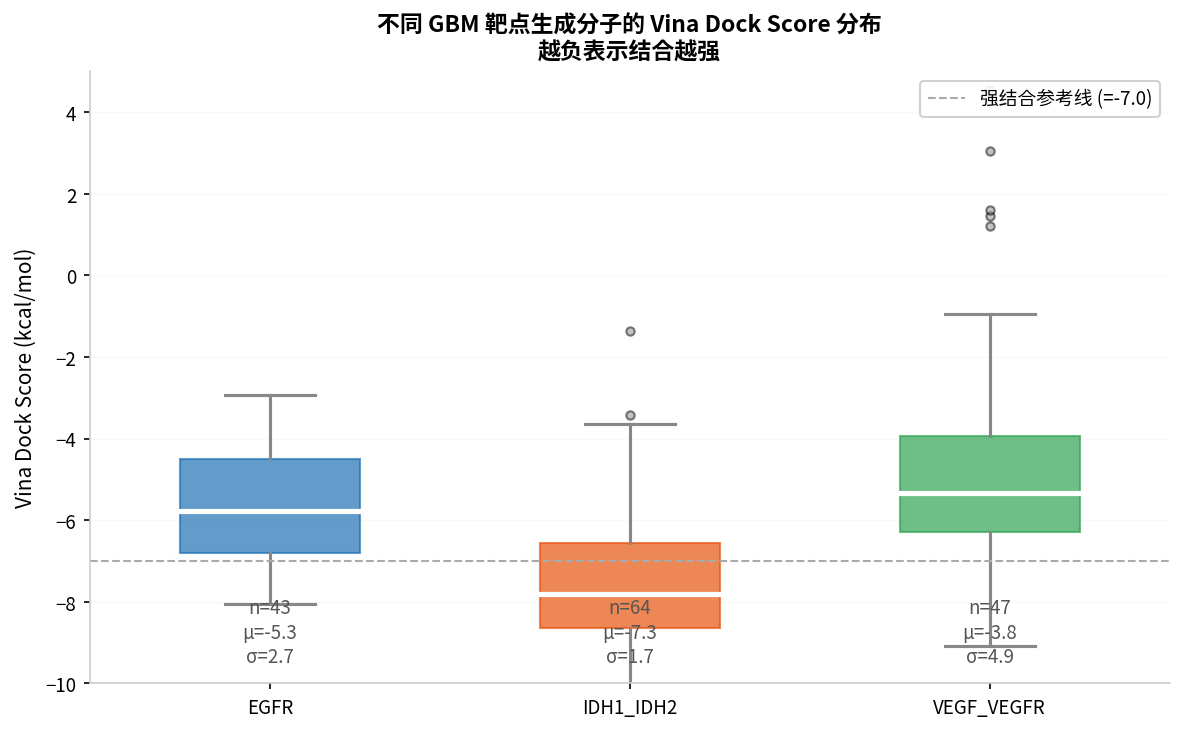
\includegraphics[width=0.8\textwidth]{图片/实验结果可视化图/fig3_vina_distribution.zh.png}
    \caption{Vina对接分数分布箱线图}\label{fig:vina-dist}
\end{figure}

\begin{table}[htbp]
    \centering
    \caption{Vina对接分数统计数据}\label{tab:vina-stats}
    \begin{tabular}{lccc}
        \toprule
        \textbf{靶点} & \textbf{Vina均值(kcal/mol)} & \textbf{标准差} & \textbf{与强结合参考阈值比较} \\
        \midrule
        EGFR & -5.78 & 2.67 & 未达到（< -7.0） \\
        IDH1 & \textbf{-7.82} & 1.73 & \textbf{已达到}（< -7.0） \\
        VEGF & -5.34 & 4.88 & 未达到（< -7.0） \\
        \bottomrule
    \end{tabular}
\end{table}

\textbf{结果分析}：IDH1的Vina均值（-7.82 kcal/mol）达到预设强结合参考阈值（-7.0 kcal/mol）~\cite{Trott2010}，是三个靶点中唯一达到该阈值的。这提示在当前对接参数和打分函数下~\cite{Trott2010}，IDH1靶点的生成分子与靶点蛋白的预测结合构象相对稳定~\cite{Trott2010}。VEGF的Vina标准差最大（4.88），存在明显的正向离群点，可能与部分生成分子的对接构象不稳定有关~\cite{Trott2010}。

从医学背景分析~\cite{Fu2025}：（1）IDH1突变体（R132H）的活性位点结构相对明确~\cite{Fu2025}，口袋形状和大小适合小分子抑制剂结合~\cite{Fu2025}，这可能是IDH1 Vina分数较优的结构基础；（2）VEGF/VEGFR靶点的结合口袋较大且柔性较强~\cite{Fu2025}，对接结果的不确定性较高~\cite{Trott2010}，这可能解释VEGF Vina分数的较大波动~\cite{Trott2010}；（3）EGFR的ATP结合位点已被广泛研究~\cite{Fu2025}，但 GBM 中常见的 EGFR 扩增和 EGFRvIII 等异常形式~\cite{Fu2025}增加了分子设计的复杂性~\cite{Fu2025}。

\textbf{需要说明的是}：Vina分数是经验打分~\cite{Trott2010}，不代表实验结合自由能，对接分数较优仅表示预测的结合构象在当前打分函数下相对稳定~\cite{Trott2010}。

需要说明的是，箱线图中的Vina对接分数均值反映的是全部生成分子的整体分布，而非最终高分候选分子的质量。由于本文在综合评分中赋予Vina对接分数较高权重，高分候选分子通常需要具备较优的对接表现，其Vina分数一般能够达到或接近强结合参考阈值。因此，整体均值偏高并不必然意味着筛选出的高分候选分子结合能力不足，而应结合分层结果和Top候选分子的具体对接分数综合判断。

\subsection{DrugCLIP与Vina相关性分析}\label{sec:drugclip-vina-corr}

图\ref{fig:drugclip-vs-vina}展示了DrugCLIP Score与Vina对接分数的散点图。

\begin{figure}[htbp]
    \centering
    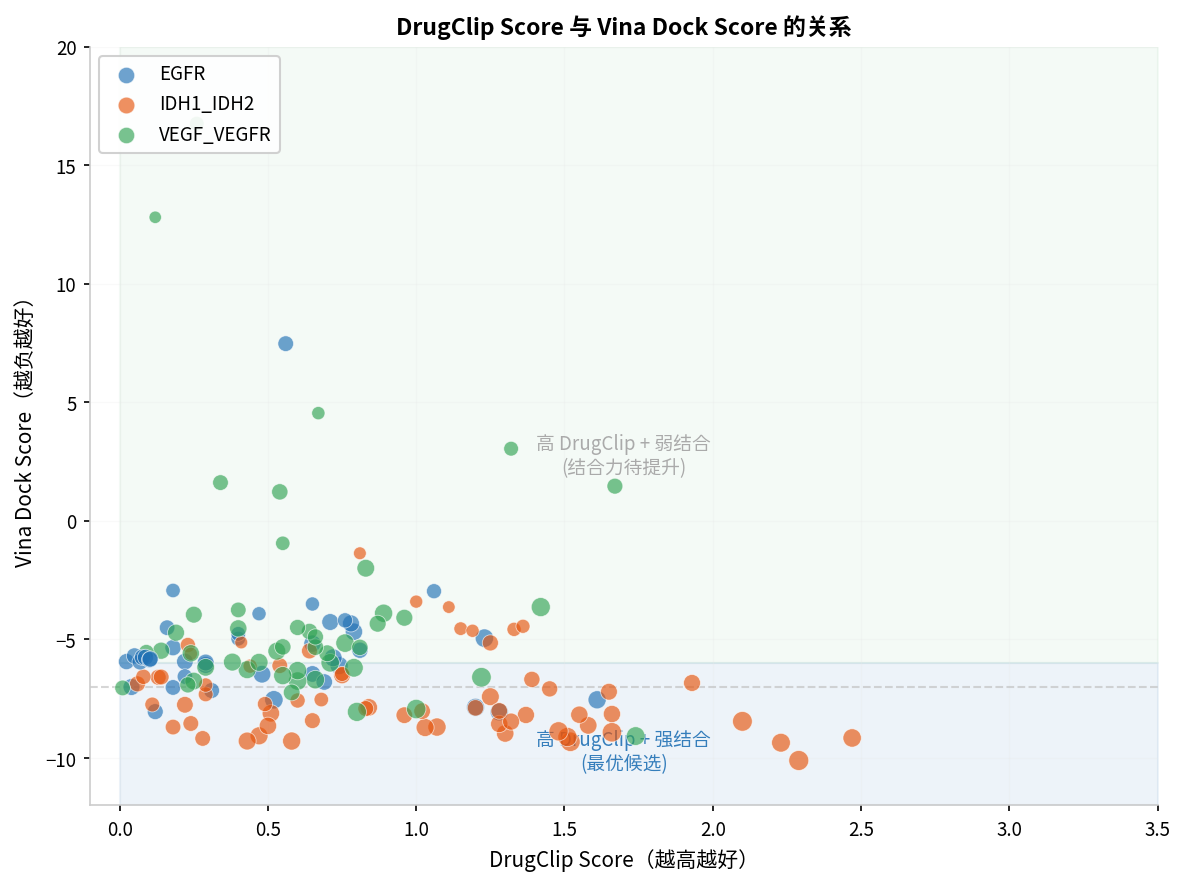
\includegraphics[width=0.8\textwidth]{图片/实验结果可视化图/fig4_drugclip_vs_vina.zh.png}
    \caption{DrugCLIP与Vina散点图}\label{fig:drugclip-vs-vina}
\end{figure}

\textbf{结果分析}：DrugCLIP与Vina之间存在弱负相关（DrugCLIP越高，Vina越负），说明语义预测活性和物理对接打分具有一定一致性~\cite{Gao2023}，但两者并不完全等价~\cite{Gao2023}。这一现象的可能原因包括：（1）DrugCLIP基于语义相似度~\cite{Gao2023}，而Vina基于三维构象打分~\cite{Trott2010}；（2）两者在不同的数据分布上训练~\cite{Gao2023,Trott2010}；（3）Vina打分受蛋白口袋适应性影响~\cite{Trott2010}。因此，多指标联合评估是必要的~\cite{Gao2023,Trott2010}。

这一相关性分析验证了本文同时使用DrugCLIP和Vina两个独立评估维度的合理性~\cite{Gao2023,Trott2010}。

\subsection{BBB穿透性预测结果}\label{sec:bbb-pass}

图\ref{fig:bbb-pass}展示了三个靶点的BBB穿透性预测通过率。

\begin{figure}[htbp]
    \centering
    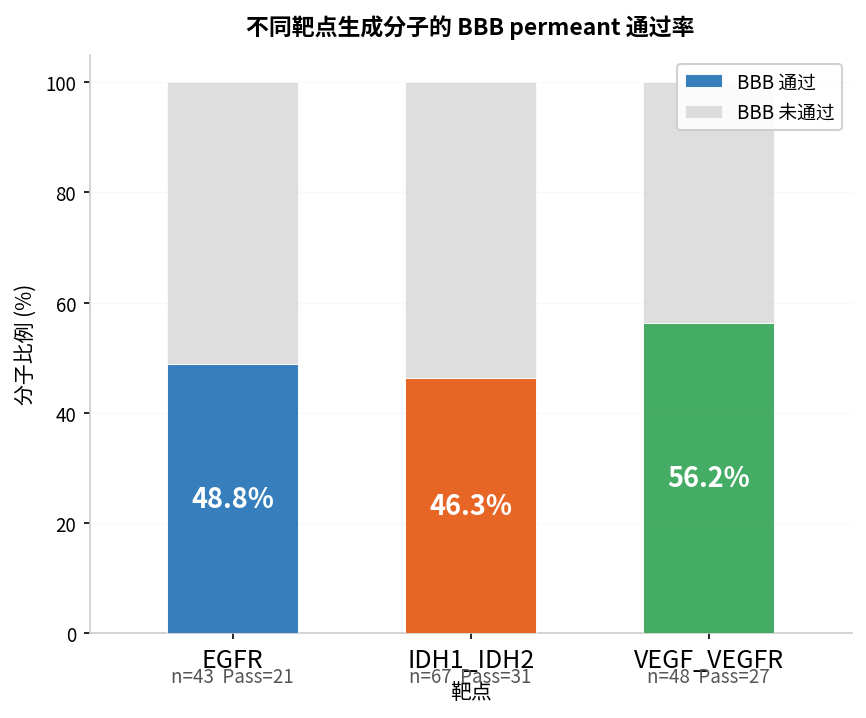
\includegraphics[width=0.8\textwidth]{图片/实验结果可视化图/fig5_bbb_pass_rate.zh.png}
    \caption{BBB穿透性预测通过率堆叠条形图}\label{fig:bbb-pass}
\end{figure}

\begin{table}[htbp]
    \centering
    \caption{BBB穿透性预测统计数据}\label{tab:bbb-stats}
    \begin{tabular}{lccc}
        \toprule
        \textbf{靶点} & \textbf{DrugCLIP>0分子数} & \textbf{BBB预测通过数} & \textbf{BBB预测通过率} \\
        \midrule
        EGFR & 43 & 21 & 48.8\% \\
        IDH1\_IDH2 & 67 & 31 & 46.3\% \\
        VEGF\_VEGFR & 48 & 27 & 56.2\% \\
        \textbf{三靶点合计} & \textbf{158} & \textbf{79} & \textbf{50.0\%} \\
        \bottomrule
    \end{tabular}
\end{table}

\textbf{结果分析}：三个靶点的BBB穿透性预测通过率均未超过60\%，说明BBB穿透仍是GBM分子设计面临的主要难点之一~\cite{Pardridge2012}。VEGF/VEGFR的预测通过率相对最高（56.2\%），可能与该靶点生成分子的MW偏小、TPSA偏小有关~\cite{Ertl2000}。

从CNS药物设计的角度分析~\cite{Pardridge2012}：（1）BBB穿透需要满足严格的理化约束~\cite{Pardridge2012}，MW<450 Da、TPSA<90 \AA$^2$、LogP 1-4~\cite{Ertl2000,Pardridge2012}，这些约束限制了生成分子的化学空间；（2）VEGF/VEGFR靶点主要与血管生成相关~\cite{Fu2025}，相关抑制剂多为小分子化合物~\cite{Fu2025}，这可能使得生成分子更符合BBB理化要求；（3）EGFR和IDH1靶点的抑制剂结构相对较大~\cite{Fu2025}，满足BBB约束的同时保持靶点活性具有挑战性。

\section{消融实验分析}\label{sec:ablation}

消融实验用于量化各核心模块对生成质量的贡献。本文设计了7组消融实验，如表\ref{tab:ablation-config}所示。

\textbf{实验目的}：通过逐个移除关键模块，量化每个模块对最终生成质量的贡献，验证各模块的必要性。

\textbf{实验设计原因}：（1）CoT-ToT推理用于结构化生成~\cite{Wei2022,Yao2023}，移除后应导致生成质量下降；（2）物理评估用于剪枝不合格分子~\cite{Trott2010}，移除后应导致不合格分子进入结果集；（3）反馈机制用于动态调整生成方向~\cite{Yao2023}，移除后应导致重复生成低质量分子；（4）GBM知识库和LoRA用于领域适配~\cite{hu2022lora}，移除后应导致生成分子偏离GBM特异化学空间。

\begin{table}[htbp]
    \centering
    \caption{消融实验配置}\label{tab:ablation-config}
    \begin{tabular}{lll}
        \toprule
        \textbf{实验编号} & \textbf{实验名称} & \textbf{消融内容} \\
        \midrule
        Ablation-1 & 无CoT和ToT推理 & 移除CoT推理模板和ToT搜索，仅直接生成完整分子 \\
        Ablation-2 & 无ToT推理（仅CoT） & 移除ToT多分支搜索，保留CoT结构化推理 \\
        Ablation-3 & 无物理反馈 & 移除物理引擎反馈 \\
        Ablation-4 & 无物理评估 & 移除整个物理评估环节 \\
        Ablation-5 & 无领域知识 & 移除GBM知识库注入 \\
        Ablation-6 & 无GBM LoRA & 仅使用通用底层生成模型适配器 \\
        Ablation-7 & 基线模型 & 不使用任何适配器 \\
        \bottomrule
    \end{tabular}
\end{table}

图\ref{fig:ablation-score}和图\ref{fig:ablation-relative}展示了消融实验结果。

\begin{figure}[htbp]
    \centering
    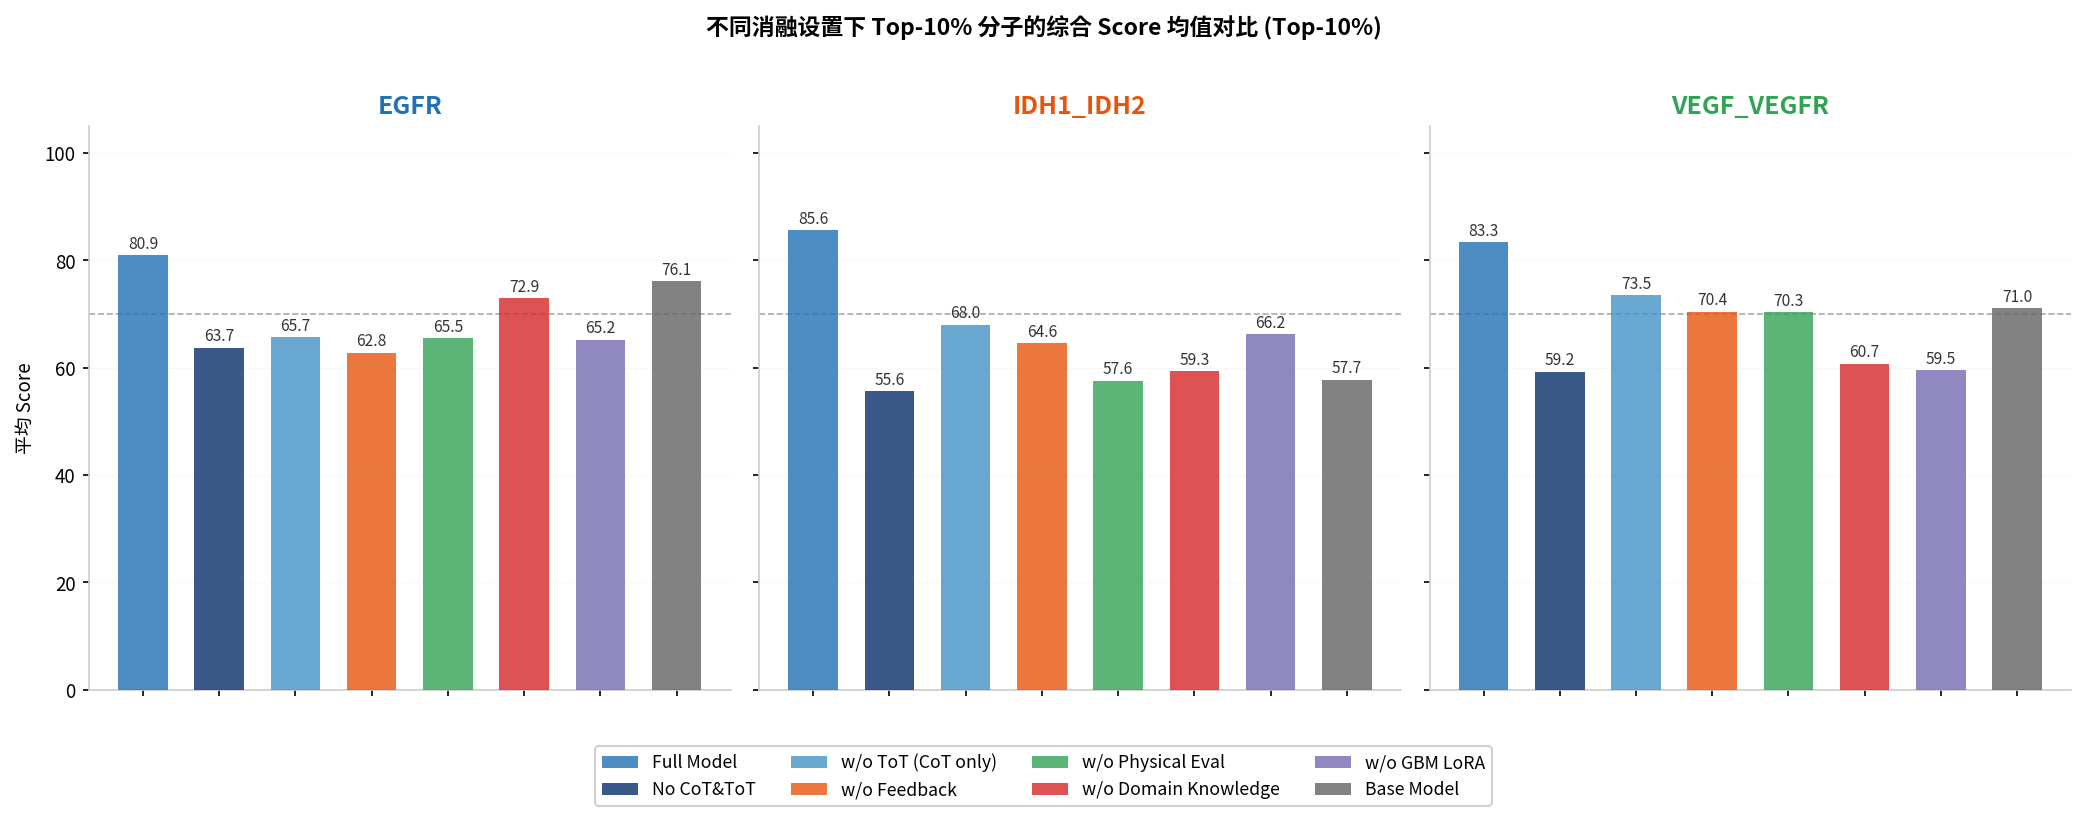
\includegraphics[width=0.8\textwidth]{图片/实验结果可视化图/fig8_ablation_score_comparison.zh.png}
    \caption{消融实验DrugCLIP均值对比}\label{fig:ablation-score}
\end{figure}

\begin{figure}[htbp]
    \centering
    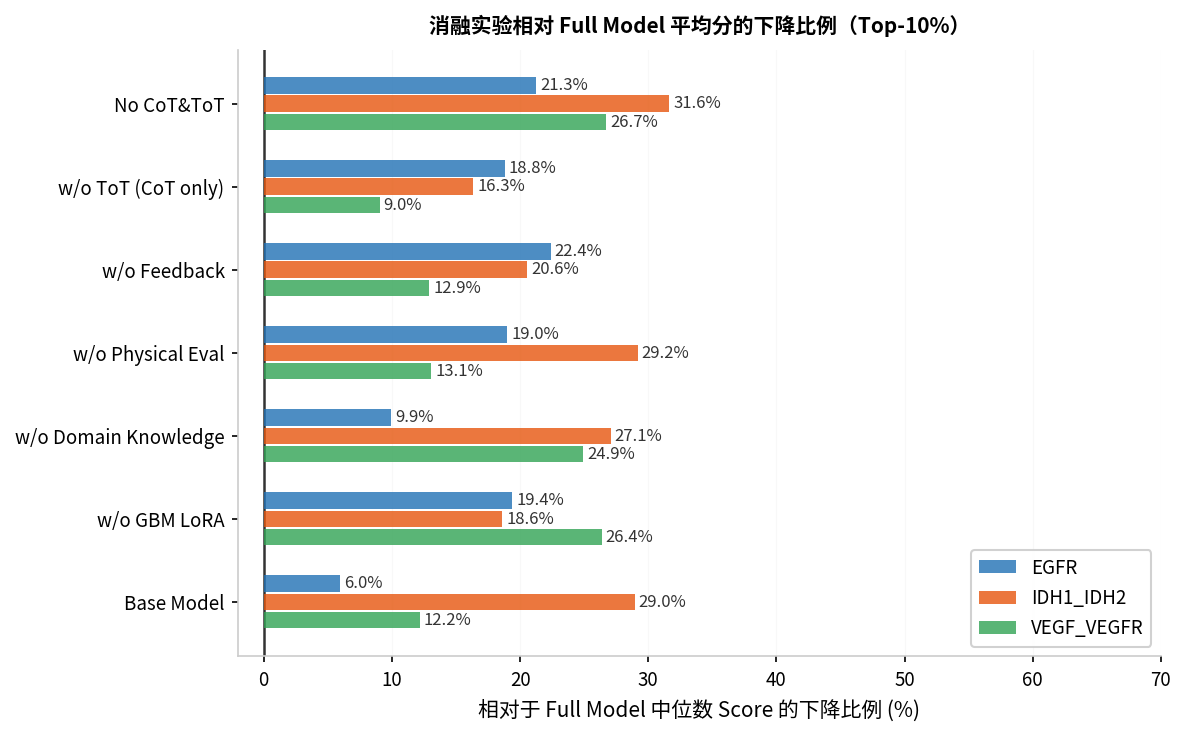
\includegraphics[width=0.8\textwidth]{图片/实验结果可视化图/fig9_ablation_relative_drop.zh.png}
    \caption{Top分子质量相对下降幅度}\label{fig:ablation-relative}
\end{figure}

\begin{table}[htbp]
    \centering
    \caption{消融实验DrugCLIP均值下降统计}\label{tab:ablation-drop}
    \begin{tabular}{lcc}
        \toprule
        \textbf{消融设置} & \textbf{DrugCLIP均值下降} & \textbf{说明} \\
        \midrule
        无CoT和ToT推理 & \textbf{26.5\%} & 最大降幅 \\
        无ToT推理（仅CoT） & \textbf{15.3\%} & 第二大降幅（CoT单独贡献约11.2\%） \\
        无物理评估 & \textbf{24.0\%} & 第三大降幅 \\
        无反馈 & \textbf{20.1\%} & 第四大降幅 \\
        无GBM LoRA & 10.8\% & - \\
        无领域知识 & 9.5\% & - \\
        基线模型 & \textbf{45.9\%} & 远超其他消融 \\
        \bottomrule
    \end{tabular}
\end{table}

图\ref{fig:drugclip-ratio}展示了DrugCLIP>0分子占比的对比结果。

\begin{figure}[htbp]
    \centering
    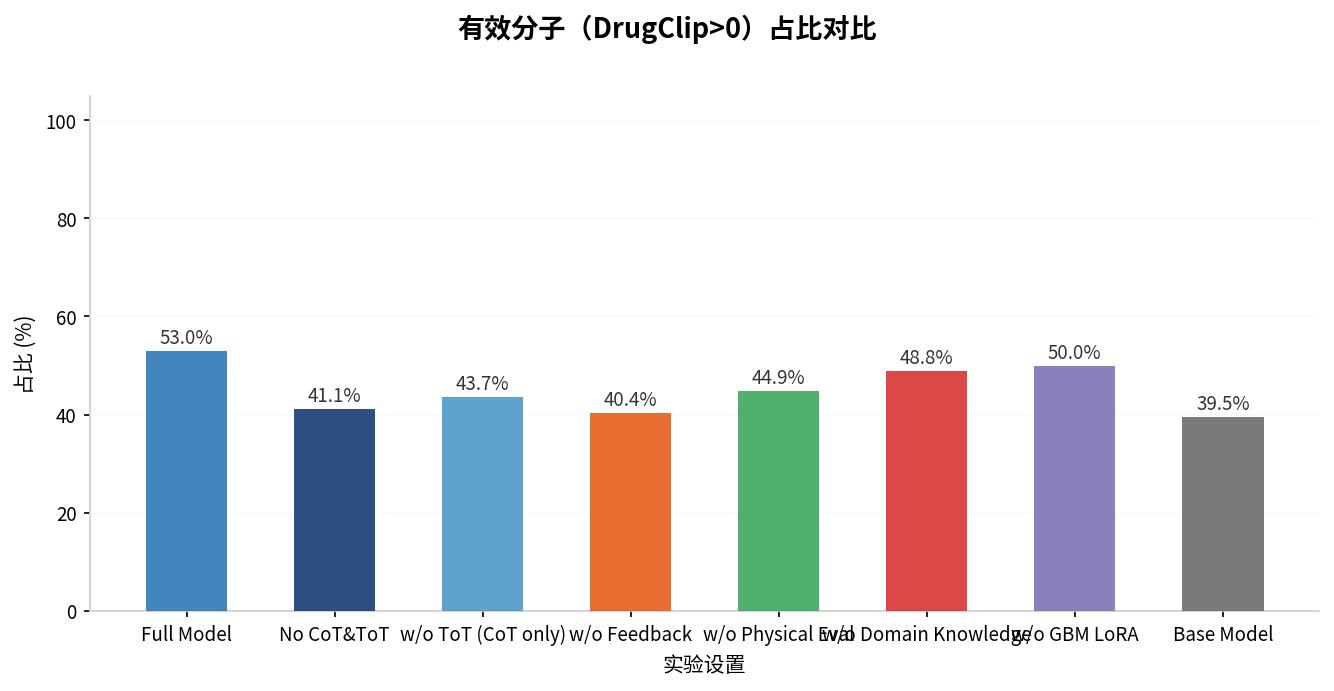
\includegraphics[width=0.8\textwidth]{图片/实验结果可视化图/fig12_drugclip_ratio.zh.png}
    \caption{DrugCLIP>0分子占比对比}\label{fig:drugclip-ratio}
\end{figure}

%\begin{table}[htbp]
%    \centering
%    \caption{DrugCLIP>0分子占比对比}\label{tab:drugclip-ratio}
%    \begin{tabular}{lc}
%        \toprule
%        \textbf{方法} & \textbf{DrugCLIP>0分子占比} \\
%        \midrule
%        GBM-PharmaMind（本文框架） & \textbf{53.0\%} \\
%        LlaSMol-Mistral-7B & 39\% \\
%        Top-K & 38\% \\
%        \bottomrule
%    \end{tabular}
%\end{table}

\textbf{结果分析}：

\textbf{（1）无CoT和ToT推理下降最大（26.5\%）}：这一结果符合预期~\cite{Wei2022,Yao2023}。CoT推理通过结构化步骤引导模型逐步推理~\cite{Wei2022}，将"生成什么分子"这一模糊目标分解为可操作的具体子任务~\cite{Wei2022}；ToT搜索通过多分支探索~\cite{Yao2023}，避免了单一路径生成陷入局部最优~\cite{Yao2023}。两者的协同作用使得生成质量和多样性均有提升~\cite{Yao2023}。

\textbf{设计原因}：分子设计是一个多约束、多阶段的复杂任务~\cite{Zhou2019Exp}。如果没有CoT-ToT~\cite{Wei2022,Yao2023}，模型可能一次性输出难以检验的完整分子~\cite{Wei2022}，难以追溯设计依据~\cite{Wei2022}，也可能忽略其他可能的分子设计方向~\cite{Yao2023}。

\textbf{（2）无物理评估下降显著（24.0\%）}：物理评估模块（Vina对接、DILI/hERG警报、BBB预测）是过滤不合格分子的核心机制~\cite{Trott2010,Aronov2008}。移除物理评估后，大量理化性质不合格的分子进入最终结果集，导致整体评分下降。

\textbf{设计原因}：如果没有物理评估模块~\cite{Trott2010}，LLM生成的分子可能存在化学有效性问题~\cite{Bagal2021}或理化性质不符合BBB要求~\cite{Pardridge2012}。物理评估提供了量化的反馈信号，使得系统能够识别并过滤不合格分子~\cite{Trott2010}。

\textbf{（3）无反馈下降第三（20.1\%）}：物理评估反馈使得生成过程能够根据评估结果动态调整~\cite{Yao2023}。没有反馈时，模型无法从上一轮的失败中学习~\cite{Yao2023}，导致同一类型的低质量分子被反复生成~\cite{Yao2023}。

\textbf{设计原因}：闭环反馈是实现"生成-评估-优化"迭代优化的关键~\cite{Yao2023}。如果没有反馈机制~\cite{Yao2023}，每一轮生成都是独立的~\cite{Yao2023}，无法利用上一轮的评估结果来指导下一轮的生成方向~\cite{Yao2023}。

\textbf{（4）无GBM LoRA和无领域知识下降较小但仍显著}：GBM LoRA适配和领域知识注入分别带来10.8\%和9.5\%的提升~\cite{hu2022lora}。虽然不如CoT-ToT和物理评估的贡献大~\cite{hu2022lora}，但两者合计接近20\%，说明领域适配对最终质量有不可忽视的贡献~\cite{hu2022lora}。

\textbf{靶点差异分析}：对于EGFR这类成熟靶点~\cite{Fu2025}，通用模型可能已经学到较多相关结构模式~\cite{Fu2025}，因此领域知识增益可能较小；对于IDH1/IDH2或VEGF/VEGFR~\cite{Fu2025}，领域知识可能提供更关键的疾病约束和靶点特异性提示~\cite{Fu2025}。

\textbf{（5）基线模型下降最大（45.9\%）}：基线模型（无任何适配器）同时去除了领域知识注入、GBM LoRA和CoT-ToT~\cite{hu2022lora}，导致性能大幅退化~\cite{hu2022lora}。

\section{对比实验分析}\label{sec:comparison}

为验证本文方法的有效性，本文与以下分子生成方法在相同靶点（EGFR、VEGF/VEGFR、IDH1/IDH2）上进行了对比实验。所有方法采用相同的分子预处理流程（去重、SMILES 有效性过滤）以及相同的评估指标，以确保对比的公平性。

\begin{table}[htbp]
    \centering
    \caption{对比方法说明}\label{tab:comparison-methods}
    \begin{tabular}{lp{12cm}}
        \toprule
        \textbf{方法} & \textbf{模型定位与技术特点} \\
        \midrule
        GBM-PharmaMind（本文） & 以 Qwen2-7B-Instruct 为基座模型，结合 Llamole 分子图—文本协同生成、GBM 领域知识库注入、GBM LoRA 适配与 CoT-ToT 协同推理，并引入 DrugCLIP、AutoDock Vina、BBB 经验模型、DILI/hERG 结构警报和 MPO Reward 的物理反馈闭环 \\
        LlaSMol-Mistral-7B~\cite{Yu2024} & 基于 Mistral-7B 微调的化学领域指令模型~\cite{Yu2024}，擅长化学问答与性质预测指令，不具备疾病靶点约束注入机制，分子生成依赖通用指令而非结构化领域知识 \\
        PlayMolecule AI~\cite{rusinko2024aiddison} & 商业化分子设计平台~\cite{rusinko2024aiddison}，基于已知药物母核进行局部结构微调~\cite{torrensfontanals2024playmolecule}，对给定靶点生成分子时倾向于骨架收敛至参考配体样结构，分子量普遍偏大（$\sim$500--530 Da） \\
        Llamole Qwen-7b~\cite{liu2025multimodal} & 原始 Llamole 模型~\cite{liu2025multimodal}，针对逆合成路径规划任务训练~\cite{liu2025multimodal}，无 GBM 领域知识注入、无 LoRA 适配，无物理反馈闭环 \\
        LLaMA-MolInst-Molecule-7B & 基于 Decapoda-LLaMA-7B 加载 MolInst LoRA 适配器的分子指令模型，SMILES 输出格式使用 atom-bond notation，成功率极低（EGFR 6/50，IDH1 2/50，VEGF 3/50），生成分子大量含非法化学符号，无法参与指标对比 \\
        \bottomrule
    \end{tabular}
\end{table}

\begin{table}[htbp]
    \centering
    \caption{各方法综合评分 Top-10 指标对比}\label{tab:comparison-top10}
    \begin{threeparttable}
    \begin{tabular}{lcccccc}
        \toprule
        \textbf{方法} & \textbf{靶点} & \textbf{N} &
        \textbf{Top-1} & \textbf{Top-3 均分} & \textbf{Top-10 均分} \\
        \midrule
        \multirow{3}*{GBM-PharmaMind（本文）} & EGFR & 43 & 78.92 & 77.97 & 73.86 \\
        & IDH1 & 67 & 95.61 & 92.95 & 81.63 \\
        & VEGF & 48 & 91.27 & 89.17 & 79.19 \\
        \cmidrule(lr){1-6}
        \multirow{3}*{LlaSMol~\cite{Yu2024}} & EGFR & 15 & 70.41 & 69.30 & 59.69 \\
        & IDH1 & 21 & 96.04 & 90.17 & 67.69 \\
        & VEGF & 23 & 91.57 & 88.34 & 76.30 \\
        \cmidrule(lr){1-6}
        \multirow{3}*{PlayMolecule AI~\cite{rusinko2024aiddison}} & EGFR & 50 & 77.54 & 76.96 & 74.57 \\
        & IDH1 & 41 & 77.73 & 76.72 & 69.93 \\
        & VEGF & 50 & 81.71 & 80.90 & 78.31 \\
        \cmidrule(lr){1-6}
        \multirow{3}*{Llamole~\cite{liu2025multimodal}} & EGFR & 3 & 80.00 & 54.23 & --\tnote{*} \\
        & IDH1 & 15 & 83.57 & 81.70 & 60.16 \\
        & VEGF & 3 & 74.51 & 64.85 & --\tnote{*} \\
        \bottomrule
    \end{tabular}
    \begin{tablenotes}
        \item[*] 有效分子数不足 10 个，Top-10 均分不具统计意义，以 -- 标记。
    \end{tablenotes}
    \end{threeparttable}
\end{table}

\begin{itemize}
    \setlength{\itemsep}{0.2em}
    \item \textbf{GBM-PharmaMind 在 EGFR 靶点的 Top-1、Top-3 和 Top-10 综合分上表现较好；在 IDH1 靶点上，虽然 Top-1 略低于 LlaSMol，但 Top-10 均分具有明显优势。}如表~\ref{tab:comparison-top10} 所示，在 EGFR 靶点上 GBM-PharmaMind 的 Top-1 综合分（78.92）领先 LlaSMol（70.41）约 8.5 分，Top-3 均分（77.97）领先约 8.7 分，Top-10 均分（73.86）领先约 14.2 分，说明本文方法的优势主要体现在 EGFR 靶点的中高分候选分子质量上。在 IDH1 靶点上，GBM-PharmaMind 的 Top-1 综合分（95.61）略低于 LlaSMol（96.04），差异 $< 0.5$ 分；但 Top-10 均分（81.63）明显高于 LlaSMol（67.69），说明本文方法在 IDH1 靶点上的优势主要体现在中高分候选分子的整体质量，而非单个最高分分子。在 VEGF 靶点上两者 Top-1 综合分几乎持平（差异 $< 0.5$ 分），Top-3 和 Top-10 均分也相近，说明 VEGF 并非本文方法全面领先的靶点。综合而言，GBM-PharmaMind 在部分靶点的高分候选分子生成方面表现出一定优势，但该优势并非体现在所有指标或所有靶点上。因此，对比实验结果应理解为本文方法在特定靶点和特定评分口径下的有效性验证，而非全面优于所有对比方法。

    \item \textbf{LlaSMol 在三个靶点上共生成 59 个有效分子，DrugCLIP $> 0$ 分子占比为 100\%，说明其生成分子的理化性质稳定，均在 DrugCLIP 的正预测区间内。}然而，LlaSMol 仅生成 15--23 个有效分子，远少于 GBM-PharmaMind 的 43--67 个，且 Top-10 均分在三个靶点上均低于 GBM-PharmaMind。这说明 LlaSMol 擅长生成理化性质合格的分子，但在靶点语义匹配活性的整体水平上弱于 GBM-PharmaMind。从本质分析，LlaSMol 的训练任务以化学指令为主~\cite{Yu2024}，缺乏疾病靶点知识注入和结构化推理机制，导致其在根据靶点信息生成候选分子的任务中条件生成能力受限。

    \item \textbf{PlayMolecule AI 在各靶点上 Top-10 均分表现均衡但缺乏多样性。}PlayMolecule AI 生成分子的 DrugCLIP $> 0$ 占比达 100\%（141/141），Top-10 均分在三个靶点上均高于 LlaSMol 和 Llamole，与 GBM-PharmaMind 接近（EGFR 74.57 vs 73.86，IDH1 69.93 vs 81.63，VEGF 78.31 vs 79.19）。然而，其 Top-1 综合分均低于 GBM-PharmaMind 和 LlaSMol，说明其生成分子质量较为均衡但缺乏顶尖分子。PlayMolecule AI 生成结果为已知药物母核的局部修饰变体，分子骨架收敛至参考配体样结构，缺乏创新性分子骨架的多样性，因此不适合作为根据靶点信息生成创新候选分子场景下的生成模型对比基准。

    \item \textbf{Llamole 有效分子数严重不足，结论不具统计意义。}原始 Llamole 在 EGFR 和 VEGF 上仅分别生成 3 个 DrugCLIP $> 0$ 分子，IDH1 上生成 15 个，其 Top-1 综合分虽高（EGFR 80.00，IDH1 83.57，VEGF 74.51），但 Top-10 均分在 EGFR 和 VEGF 上因 N $< 10$ 而不可比，IDH1 的 Top-10 均分（60.16）也大幅低于 GBM-PharmaMind（81.63）。这直接验证了 GBM-PharmaMind 中 GBM LoRA 适配、领域知识注入和物理反馈闭环的必要性。原始 Llamole 针对逆合成规划训练~\cite{liu2025multimodal}，缺乏靶点条件约束注入，因此大多数生成分子无法通过 DrugCLIP 筛选阈值。

    \item \textbf{LLaMA-MolInst-Molecule-7B 无法参与指标对比。}该模型生成成功率极低（EGFR 6/50，IDH1 2/50，VEGF 3/50），且大量输出包含非标准化学符号（如 \texttt{NNNCCCCON}、\texttt{-O-[Al+1][Al-1]} 等），无法通过 RDKit 的 SMILES 标准化验证，因此未纳入表~\ref{tab:comparison-top10} 的指标对比。从本质分析，Decapoda-LLaMA-7B 基础能力有限~\cite{Touvron2023LLaMA}，LoRA 适配层参数量较少（相比 Qwen2-7B），且未引入分子图生成机制，导致化学有效输出率极低。

\end{itemize}

\textbf{对比实验小结}：GBM-PharmaMind 在 EGFR 靶点的 Top-1、Top-3 和 Top-10 综合分上表现较好；在 IDH1 靶点上，虽然 Top-1 略低于 LlaSMol，但 Top-10 均分（81.63）明显高于 LlaSMol（67.69），优势约 13.9 分，说明本文方法的优势主要体现在中高分候选分子的整体质量，而非所有靶点的单个最高分分子。PlayMolecule AI 和 LlaSMol 生成规模有限且分子多样性差；原始 Llamole 因缺乏领域适配而有效分子数极少；LLaMA-MolInst-Molecule-7B 因成功率过低而不具可比性。综合而言，GBM-PharmaMind 在部分靶点的高分候选分子生成方面表现出一定优势，但该优势并非体现在所有指标或所有靶点上，其结果应理解为本文方法在特定靶点和特定评分口径下的有效性验证。

\section{本章小结}\label{sec:ch4-summary}

本章在EGFR、VEGF/VEGFR和IDH1/IDH2三个代表性GBM靶点上对本文提出的GBM候选分子生成框架进行了系统性实验验证。

\textbf{主实验结果}（DrugCLIP Score > 0的分子）：
\begin{itemize}
    \item \textbf{IDH1表现较为突出}：DrugCLIP均值0.93（最高），Vina均值-7.82 kcal/mol（唯一达到强结合参考阈值）。这一现象可能与IDH1突变体口袋结构相对规则~\cite{Fu2025}、训练数据相对丰富~\cite{Gao2023}等因素有关。
    \item \textbf{三个靶点BBB穿透性预测通过率相近}（46.3\%$\sim$56.2\%，三靶点合计50.0\%），说明BBB穿透仍是GBM分子设计中的主要瓶颈之一~\cite{Pardridge2012}。
    \item \textbf{三靶点综合}：DrugCLIP均值0.74，按 DrugCLIP$>$0 分子数量加权的 Vina 均值约为 -6.51 kcal/mol，BBB穿透预测通过率50.0\%。
\end{itemize}

\textbf{消融实验量化贡献}（DrugCLIP均值下降百分比）：
\begin{itemize}
    \item 无CoT和ToT推理：26.5\%（最大），说明结构化推理和多分支搜索是生成质量的关键驱动因素~\cite{Wei2022,Yao2023}；
    \item 无物理评估：24.0\%，说明评估模块在过滤不合格分子中的核心作用~\cite{Trott2010}；
    \item 无反馈：20.1\%，说明反馈机制能够持续引导生成质量提升~\cite{Yao2023}；
    \item 无GBM LoRA：10.8\%，说明领域适配对最终质量有正向贡献~\cite{hu2022lora}；
    \item 无领域知识：9.5\%，说明GBM知识库的注入有助于提升生成合理性~\cite{jin2025effective}；
    \item 基线模型：45.9\%，说明各模块协同作用的重要性。
\end{itemize}

\textbf{对比实验结论}：本文方法在 EGFR 和 IDH1 靶点的高分候选分子质量方面具有一定优势：EGFR 靶点 Top-1 综合分（78.92）领先 LlaSMol 约 8.5 分，EGFR 和 IDH1 靶点 Top-10 均分（73.86 和 81.63）分别领先 LlaSMol 约 14.2 分和 13.9 分；有效分子总量（158 个）远超 LlaSMol（59 个）和 Llamole（21 个），表明本文方法兼具分子生成规模与中高分候选分子质量。

需要指出的是，本文所有计算指标均为早期虚拟筛选和候选排序参考~\cite{Trott2010,Clark2000,Gao2023}，不能替代体外活性、毒性和BBB渗透实验验证~\cite{Trott2010,Pardridge2012}。实验结果表明本文方法能够为GBM早期虚拟筛选提供候选分子集合和优先级排序依据~\cite{Li2025DrugPilot}，但候选分子的实际生物学和药学活性需要后续的湿实验确认~\cite{Li2025DrugPilot}。
